%%%%%%%%%%%%%%%%%%%%%%%%%%%%%%%%%%%%%%%%%%%%%%%%%%%%%%%%%%%%
%%  This Beamer template was created by Cameron Bracken.
%%  Anyone can freely use or modify it for any purpose
%%  without attribution.
%%
%%  Last Modified: January 9, 2009
%%

\documentclass[xcolor=x11names,compress]{beamer}

%% General document %%%%%%%%%%%%%%%%%%%%%%%%%%%%%%%%%%

\usepackage{graphicx}
\usepackage{tikz}
\usetikzlibrary{decorations.fractals}
%%%%%%%%%%%%%%%%%%%%%%%%%%%%%%%%%%%%%%%%%%%%%%%%%%%%%%
\graphicspath{{./Pictures/}}

%% Beamer Layout %%%%%%%%%%%%%%%%%%%%%%%%%%%%%%%%%%
\useoutertheme[subsection=false,shadow]{miniframes}
\useinnertheme{default}
\setbeamertemplate{navigation symbols}{}
\setbeamertemplate{blocks}[rounded][shadow=false]


\setbeamertemplate{footline}
{
\begin{beamercolorbox}[wd=\paperwidth,ht=0.3ex,dp=1.125ex,%
	 leftskip=.3cm,rightskip=.3cm plus1fil]{upper separation line foot}
\end{beamercolorbox} %

\begin{beamercolorbox}[wd=\paperwidth,ht=2.5ex,dp=1.125ex,%
	 leftskip=.3cm,rightskip=.3cm plus1fil]{footlinecolor}%
        \usebeamerfont{section in head/foot}%
	\color{gray} \insertshortauthor\hfill\insertpagenumber{} of \insertpresentationendpage{}

    \end{beamercolorbox}

}



\usefonttheme{serif} % default family is serif
\usepackage{fontspec}
\defaultfontfeatures{Numbers=OldStyle}
\setmainfont{Minion Pro}


\setbeamerfont{title like}{shape=\scshape}
\setbeamerfont{frametitle}{shape=\scshape}


\setbeamercolor*{lower separation line head}{bg=DodgerBlue3}
\setbeamercolor*{upper separation line foot}{bg=DodgerBlue3}

\setbeamercolor*{footlinecolor}{fg=black,bg=black!10}
\setbeamercolor*{normal text}{fg=black,bg=white} 
\setbeamercolor*{alerted text}{fg=Firebrick1} 
\setbeamercolor*{example text}{fg=DarkOliveGreen1} 
\setbeamercolor*{structure}{fg=black} 
\setbeamercolor*{palette tertiary}{fg=black,bg=black!10} 
\setbeamercolor*{palette quaternary}{fg=black,bg=black!10} 

\renewcommand{\(}{\begin{columns}}
\renewcommand{\)}{\end{columns}}
\newcommand{\<}[1]{\begin{column}{#1}}
\renewcommand{\>}{\end{column}}



%%%%%%%%%%%%%%%%%%%%%%%%%%%%%%%%%%%%%%%%%%%%%%%%%%




\begin{document}

\title{Design and Usability Testing of a Mobile Phone-Based Patient Management System for Women in Rural Kenya}
\author[Amogh Karnik]{
	Amogh Karnik\\
	{\it M.Sc. Candidate}\\
}
\institute[DGHI]{Duke Global Health Institute}
\date{\today}
%%%%%%%%%%%%%%%%%%%%%%%%%%%%%%%%%%%%%%%%%%%%%%%%%%%%%%
%%%%%%%%%%%%%%%%%%%%%%%%%%%%%%%%%%%%%%%%%%%%%%%%%%%%%%

\begin{frame}
\titlepage
\end{frame}

\begin{frame}{Overview}
\tableofcontents
\end{frame}


%%%%%%%%%%%%%%%%%%%%%%%%%%%%%%%%%%%%%%%%%%%%%%%%%%%%%%
%%%%%%%%%%%%%%%%%%%%%%%%%%%%%%%%%%%%%%%%%%%%%%%%%%%%%%
\section{Introduction}
\subsection{Maternal Mortality}

\begin{frame}

\begin{alertblock}{Every day, 800 women die of pregnancy-related complications around the world.}

\end{alertblock}
\pause
\begin{alertblock}{The most common causes of maternal death are hemorrhage and infection.}
\end{alertblock}
\pause
\begin{alertblock}{Most of these deaths take place during or within the first few days after childbirth.}
\end{alertblock}
\pause
\begin{alertblock}{In Sub-Saharan Africa, 1 of 16 women will die of pregnancy-related complications.}
\end{alertblock}
\end{frame}


\begin{frame}
\begin{center}
Most maternal deaths are avoidable.
\end{center}
\end{frame}



%%%%%%%%%%%%%%%%%%%%%%%%%%%%%%%%%%%%%%%%%%%%%%%%%%%%%%
%%%%%%%%%%%%%%%%%%%%%%%%%%%%%%%%%%%%%%%%%%%%%%%%%%%%%%
\section{Methods}
\subsection{Setting}
\begin{frame}
\begin{figure}
\centerline{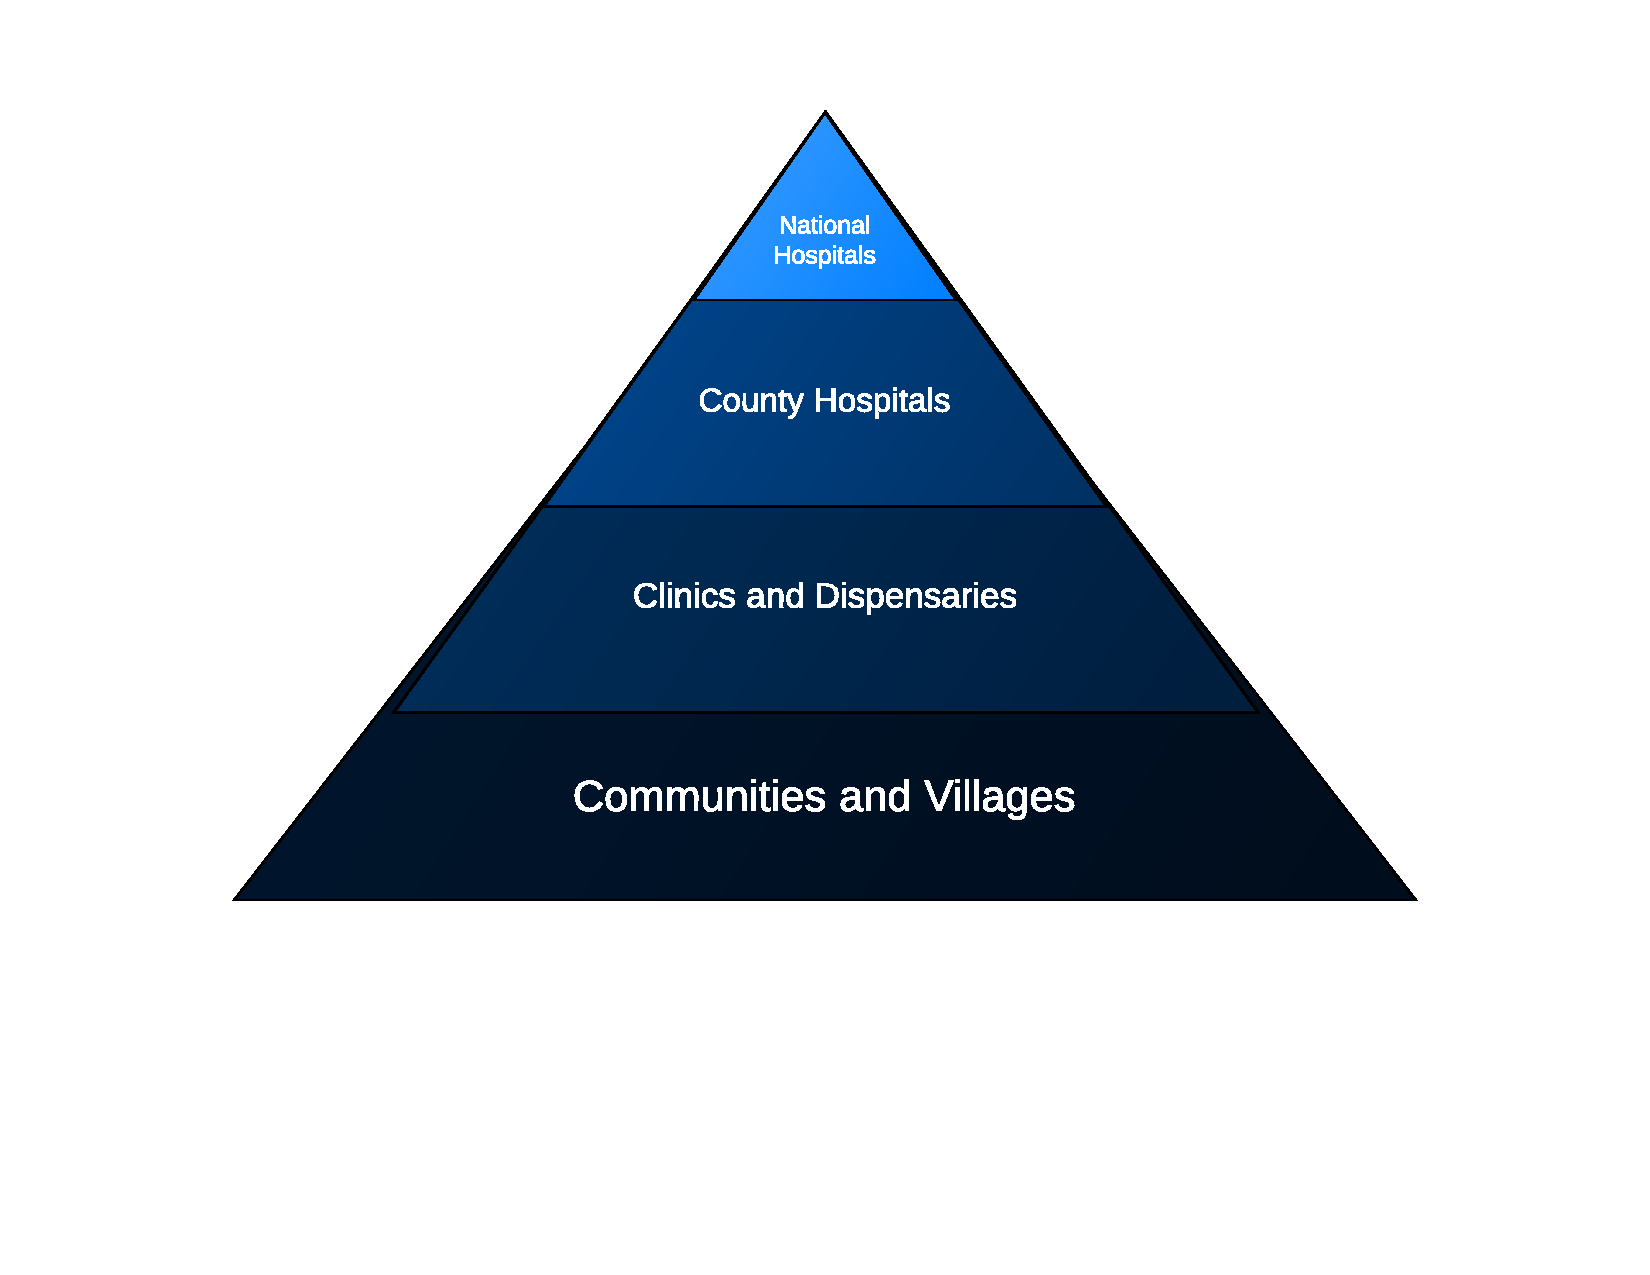
\includegraphics[scale=0.45]{health-system}}l
\end{figure}
\end{frame}

\begin{frame}{Research Site}
Specifics about Sinoko clinic, Ndivisi, Bungoma County
\end{frame}

\subsection{Human-Centered Design}
\begin{frame}{Human-Centered Design}
Explanation of the HCD framework.
\end{frame}

\begin{frame}{Hear Phase}
This is the hear phase.
\end{frame}

\begin{frame}{Create Phase}
This is the create phase.
\end{frame}

\begin{frame}{Deliver Phase}
This is the deliver phase.
\end{frame}


%%%%%%%%%%%%%%%%%%%%%%%%%%%%%%%%%%%%%%%%%%%%%%%%%%%%%%
%%%%%%%%%%%%%%%%%%%%%%%%%%%%%%%%%%%%%%%%%%%%%%%%%%%%%%
\section{Results}
\subsection{Qualitative Results}
\begin{frame}{Create Phase}
These are the results of the create phase.
\end{frame}

\subsection{Quantitative Results}
\begin{frame}{Deliver Phase}
\end{frame}

%%%%%%%%%%%%%%%%%%%%%%%%%%%%%%%%%%%%%%%%%%%%%%%%%%%%%%
%%%%%%%%%%%%%%%%%%%%%%%%%%%%%%%%%%%%%%%%%%%%%%%%%%%%%%
\section{Discussion}
\subsection{Frame 1}
\begin{frame}{Frame 1}

\end{frame}



%%%%%%%%%%%%%%%%%%%%%%%%%%%%%%%%%%%%%%%%%%%%%%%%%%%%%%
%%%%%%%%%%%%%%%%%%%%%%%%%%%%%%%%%%%%%%%%%%%%%%%%%%%%%%
\end{document}